\documentclass[12pt,landscape]{article}
\usepackage{pgfgantt}
\usepackage{tikz}
\usepackage[letterpaper, landscape, margin=0.5in]{geometry}
\begin{document}
\begin{flushleft}
Adam Frazee\\
CSE 201\\
Dr.Sobel\\
2/10/2016\\
\end{flushleft}
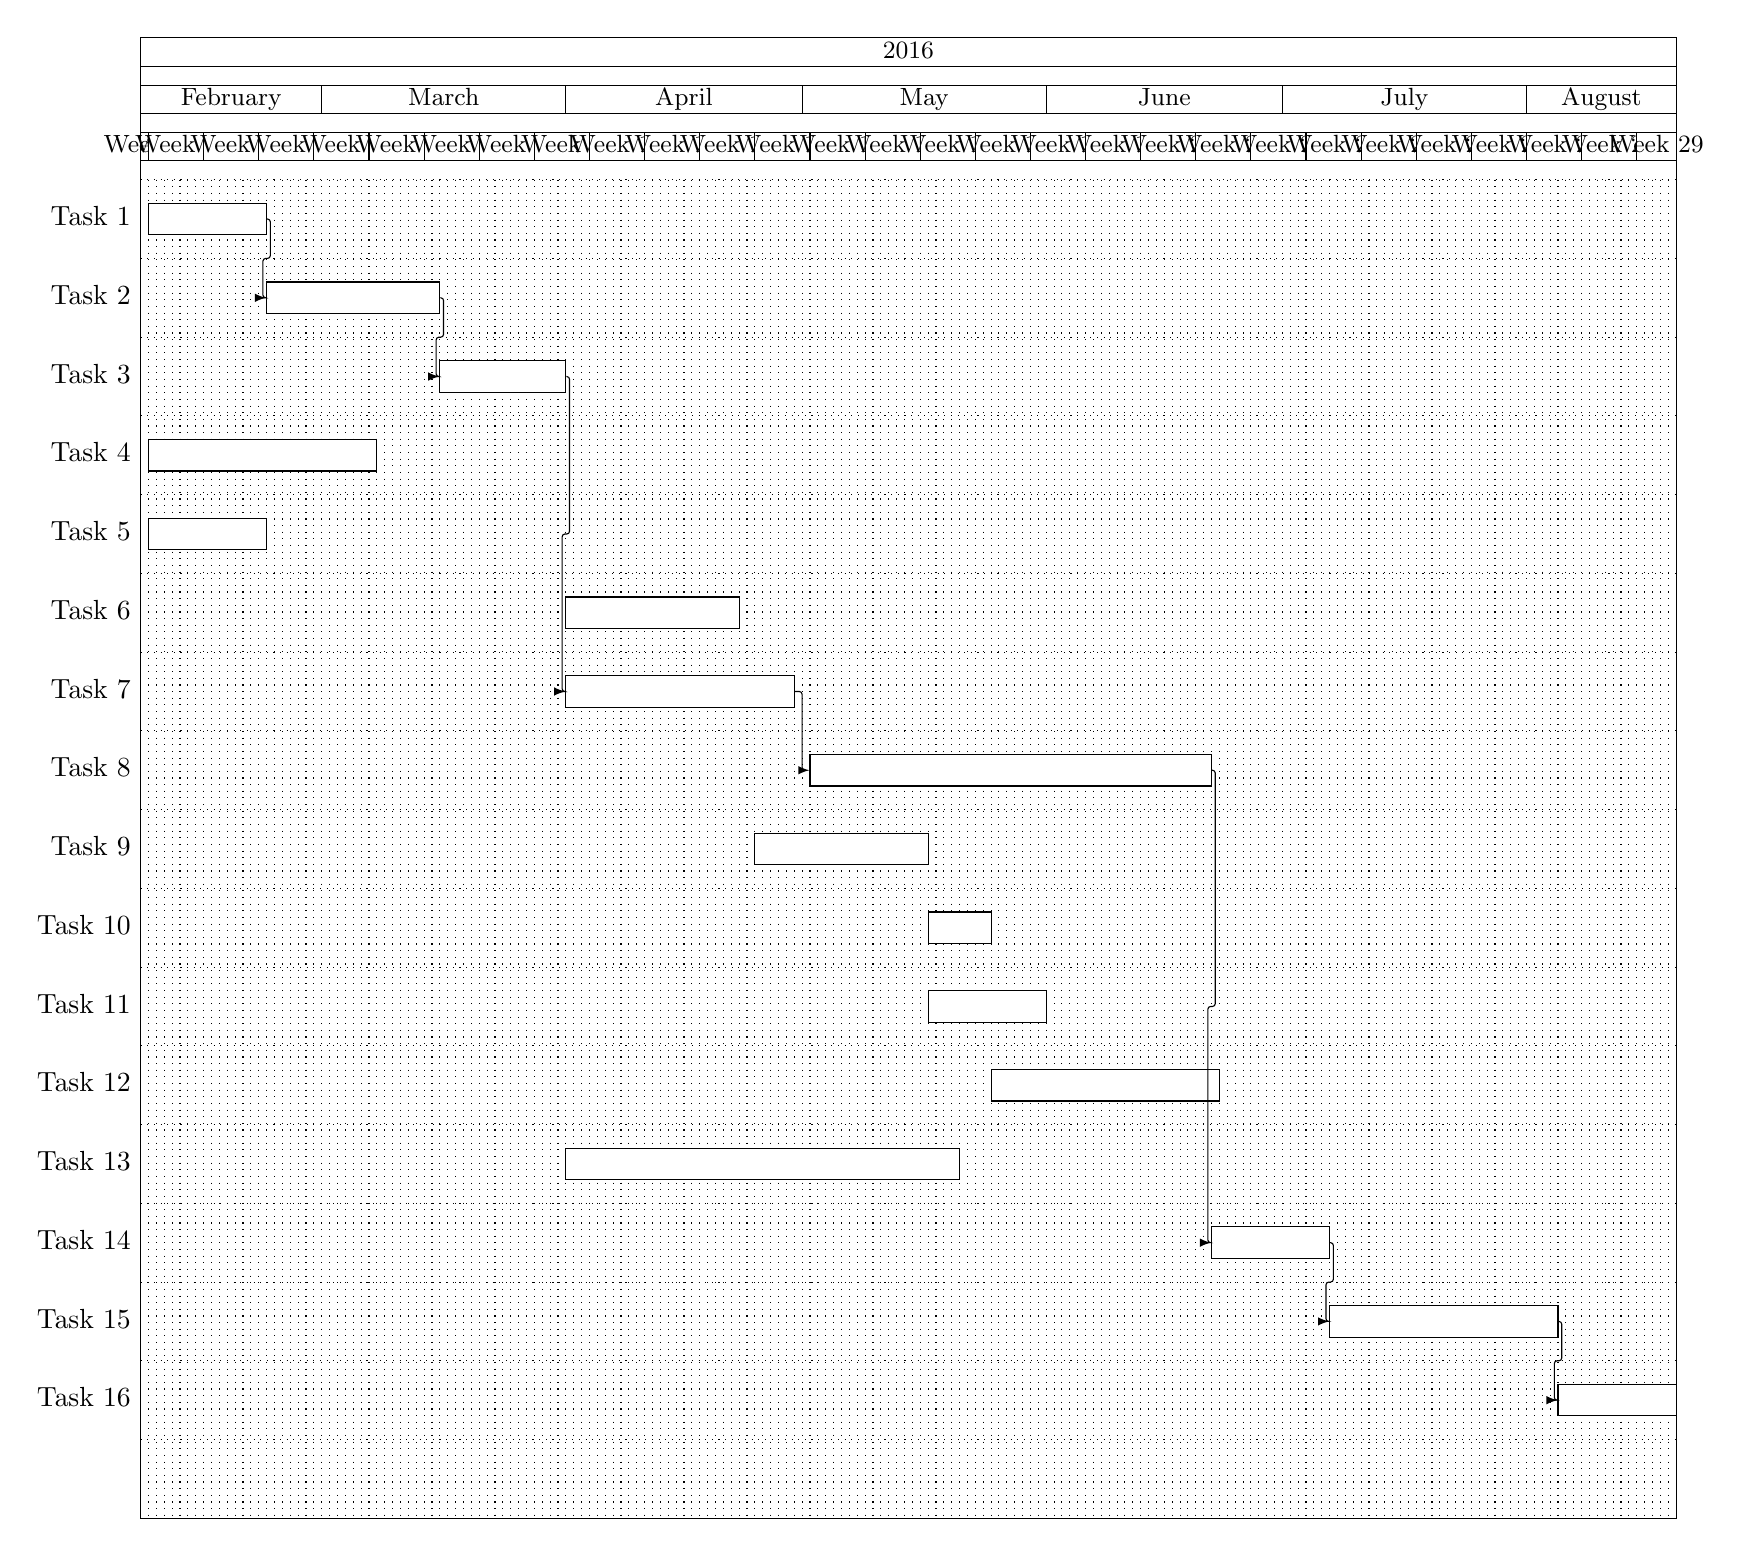
\begin{tikzpicture}
\begin{ganttchart}[
time slot format=isodate,
x unit=.1cm,
y unit title=.6cm,
y unit chart=1cm,
vgrid, hgrid
]{2016-02-07}{2016-08-19}
\gantttitlecalendar{year, month=name, week} \\


\ganttbar{Task 1}{2016-02-08}{2016-02-22} \\
\ganttbar{Task 2}{2016-02-23}{2016-03-15} \\
\ganttbar{Task 3}{2016-03-16}{2016-03-31} \\
\ganttbar{Task 4}{2016-02-08}{2016-03-07} \\
\ganttbar{Task 5}{2016-02-08}{2016-02-22} \\
\ganttbar{Task 6}{2016-04-01}{2016-04-22} \\
\ganttbar{Task 7}{2016-04-01}{2016-04-29} \\
\ganttbar{Task 8}{2016-05-02}{2016-06-21} \\
\ganttbar{Task 9}{2016-04-25}{2016-05-16} \\
\ganttbar{Task 10}{2016-05-17}{2016-05-24} \\
\ganttbar{Task 11}{2016-05-17}{2016-05-31} \\
\ganttbar{Task 12}{2016-05-25}{2016-06-22} \\
\ganttbar{Task 13}{2016-04-01}{2016-05-20} \\
\ganttbar{Task 14}{2016-06-22}{2016-07-06} \\
\ganttbar{Task 15}{2016-07-07}{2016-08-04} \\
\ganttbar{Task 16}{2016-08-05}{2016-08-19} \\

\ganttlink{elem0}{elem1}
\ganttlink{elem1}{elem2}
\ganttlink{elem2}{elem6}
\ganttlink{elem6}{elem7}
\ganttlink{elem7}{elem13}
\ganttlink{elem13}{elem14}
\ganttlink{elem14}{elem15}





\end{ganttchart}
\end{tikzpicture}


\end{document}